% HW Template for CS 6150, taken from https://www.cs.cmu.edu/~ckingsf/class/02-714/hw-template.tex
%
% You don't need to use LaTeX or this template, but you must turn your homework in as
% a typeset PDF somehow.
%
% How to use:
%    1. Update your information in section "A" below
%    2. Write your answers in section "B" below. Precede answers for all 
%       parts of a question with the command "\question{n}{desc}" where n is
%       the question number and "desc" is a short, one-line description of 
%       the problem. There is no need to restate the problem.
%    3. If a question has multiple parts, precede the answer to part x with the
%       command "\part{x}".
%    4. If a problem asks you to design an algorithm, use the commands
%       \algorithm, \correctness, \runtime to precede your discussion of the 
%       description of the algorithm, its correctness, and its running time, respectively.
%    5. You can include graphics by using the command \includegraphics{FILENAME}
%
\documentclass[11pt]{article}
\usepackage{tikz}
\usetikzlibrary{positioning}
\newdimen\nodeDist
\nodeDist=20mm
\usepackage{amsmath,amssymb,amsthm}
\usepackage{graphicx}
\usepackage[margin=1in]{geometry}
\usepackage{fancyhdr}
\usepackage{longtable}
\setlength{\parindent}{0pt}
\setlength{\parskip}{5pt plus 1pt}
\setlength{\headheight}{13.6pt}
\newcommand\question[2]{\vspace{.25in}\hrule\textbf{#1: #2}\vspace{.5em}\hrule\vspace{.10in}}
\renewcommand\part[1]{\vspace{.10in}\textbf{(#1)}}
\newcommand\approach{\vspace{.10in}\textbf{Approach: }}
\newcommand\algorithm{\vspace{.10in}\textbf{Algorithm: }}
\newcommand\assumption{\vspace{.10in}\textbf{Assumption: }}
\newcommand\correctness{\vspace{.10in}\textbf{Correctness: }}
\newcommand\runtime{\vspace{.10in}\textbf{Running time: }}
\pagestyle{fancyplain}
\lhead{\textbf{\NAME\ (\UID)}}
\chead{\textbf{HW\HWNUM}}
\rhead{CS 6350, \today}
\begin{document}\raggedright
%Section A==============Change the values below to match your information==================
\newcommand\NAME{Aishwarya Asesh}  % your name
\newcommand\UID{u1063384}     % your utah UID
\newcommand\HWNUM{6}              % the homework number
%Section B==============Put your answers to the questions below here=======================

% no need to restate the problem --- the graders know which problem is which,
% but replacing "The First Problem" with a short phrase will help you remember
% which problem this is when you read over your homeworks to study.

Collaborators: Sarvagya Shastri, Vinod Dubey\\
Referrences: Lecture Notes UC Berkeley\\

\question{1}{Warm up: Probabilities}
\part{1} 
For this particular question we are given that: \newline
$P(A_1) = P(A_2) = P(A_1 | A_2) = {1}/{2}$\\
We know from the conditional probability theorem:\\
$P(A_1 , A_2) = P(A_1 | P(A_2))P(A_2) = {1}/{2} \times {1}/{2} = {1}/{4}$\\
After computing the product of single probabilities, we can observe that:\\
$P(A_1)P(A_2) = {1}/{2} \times {1}/{2} = {1}/{4}$\\
If we use the results computed in these previous two equations, we can observe that:\\
$P(A_1 , A_2) = P(A_1 | P(A_2))P(A_2) = {1}/{2} \times {1}/{2} = {1}/{4} = P(A_1)P(A_2)$\\
Therefore we can say that, $A_1$ and $A_2$ are not dependent.

\part{2}
We have been given that, $A_1$ ,$A_2$ and $A_3$ are all mutually exclusive\\
We can observe that\\
$P(A_i) = {1}/{3}$ \& $P(A_4 | A_i) = {i}/{6}$\\ Thus we can see the probability definiton as folllows:\\
$P(A_1) = P(A_2) = P(A_3) = P(A_4) = {1}/{3}$\\
$P(A_4|A_{i=1}) = {1}/{6}$\\
$P(A_4|A_{i=2}) = {1}/{3}$\\
$P(A_4|A_{i=3}) = {1}/{2}$\\
We can now take into account the total probability theorem to compute the term $P(A_4)$:\\  
$P(A_4) = P(A_1)P(A_4|A_1) + P(A_2)P(A_4|A_2) + P(A_3)P(A_4|A_3)$\\
$P(A_4) = ({1}/{3}\times {1}/{6}) + ({1}/{3} \times {1}/{3}) + ({1}/{3}\times {1}/{2}) = {1}/{3}$\\
Thus, we get the required answer.\\

\part{3}
As per the given condition, two heads can show up in only one case when we toss the dice and it shows up a number more than or equal to two. The case for one independent toss for an unbiased coin, the probabilities are as follows:\\
$P(H) = {1}/{2}$ \& $P(T) = {1}/{2}$\\
The whole statement of the problem is based on what value of n is given by the dice.\\
Therefore probability that the number of heads we get after tossing coin will be equal to two is:\\
$P(H=2) = \sum_{n=2}^6P(H=2|n)P(n)$\\
Which on further expansion gives the equation as:\\
$P(H=2) = P(H=2|n=2)P(n=2) + P(H=2|n=3)P(n=3) + P(H=2|n=4)P(n=4) + P(H=2|n=5)P(n=5 ) + P(H=2|n=6)P(n=6)$\\

At this point, for a particular $n$ value in which case $n$ is greater than equal to 2, we can say the probability of getting exact 2 heads can be written as:\\ 
$\binom{n}{2} P(H)^2P(T)^{n-2}$ = $\binom{n}{2}\bigg ({1}/{2} \bigg )^2 \bigg ( {1}/{2} \bigg)^{n-2} = \binom{n}{2}\bigg ( {1}/{2} \bigg)^n$\\

We can observe here that as we have been given dice that is unbiased and fair, therefore the probability of getting an n ranging from 1,2,3,4,5,6 can have the exact same probability. Therefore,
$P(n=2) = P(n=3) = P(n=4) = P(n=5) = P(n=6) = {1}/{6}$\\
Thus, using the above statement in the equation to get the probability for getting exact 2 heads:\\
$P(H=2) = \binom{2}{2}\bigg ( {1}/{2} \bigg )^2{1}/{6} + \binom{3}{2}\bigg ( {1}/{2} \bigg )^3{1}/{6} + \binom{4}{2}\bigg ( {1}/{2} \bigg )^4{1}/{6} + \binom{5}{2}\bigg ( {1}/{2} \bigg )^5{1}/{6} + \binom{6}{2}\bigg ( {1}/{2} \bigg )^6{1}/{6}$\\
$P(H=2) = \bigg ( {1}/{2} \bigg )^2{1}/{6} + 3\bigg ({1}/{2} \bigg )^3{1}/{6} + 6\bigg ({1}/{2} \bigg )^4{1}/{6} + 10\bigg ({1}/{2} \bigg )^5{1}/{6} + 15\bigg ({1}/{2} \bigg )^6{1}/{6}$\\
That can be further written as:\\
$P(H=2) = \dfrac{1}{6} \bigg (\bigg ({1}/{2} \bigg )^2 + 3\bigg ({1}/{2} \bigg )^3 + 6\bigg ({1}/{2} \bigg )^4 + 10\bigg ({1}/{2} \bigg )^5 + 15\bigg ({1}/{2} \bigg )^6 \bigg ) = {33}/{128}$\\
Thus, we have the required answer.\\

\part{4}
We are given, the following terms:\\ 
$P(A_1) = a_1$ and $P(A_2) = a_2$.\\
Using the conditional probabiity, we can mention that:\\ 
$P(A_1 | A_2) = {P(A_1 \cap A_2)}/{P(A_2)} = {P(A_1) + P(A_2) - P(A_1 \cup A_2)}/{P(A_2)}$\\
At this point we see that, $P(A_1 \cup A_2)$ is less than or equal to 1. Hence, we get the values:\\
$P(A_1 | A_2) = \dfrac{P(A_1) + P(A_2) - P(A_1 \cup A_2)}{P(A_2)}$ is greater than or equal to $\dfrac{P(A_1) + P(A_2) - 1}{P(A_2)}$\\
Substituting the probability values in this equation, we can infer:\\
$P(A_1 | A_2) = \dfrac{P(A_1) + P(A_2) - P(A_1 \cup A_2)}{P(A_2)}$ is greater than or equal to $\dfrac{a_1 + a_2 - 1}{a_2}$\\

\part{5}\textbf{(A)} \textbf{Required Proof:} As it is given, we assume that $A_1$ and $A_2$ are independent events.\\
In this case $A_1$ and $A_2$ are discrete random variables.\\
Thus, accordingly we can write the expectation of $A_1$ =
$E[A_1] = \sum_{a_1} a_1P(A_1 = a_1)$\\
in which case $a_1$ denotes the particular values that $A_1$ can take as input and $P(a_2)$ denotes their respective probabilities.\\ 
In a same way, we can observe:\\
$E[A_2] = \sum_{a_2} a_2P(A_2 = a_2)$\\
Thus, we can expand this further in a way such as:\\
$E[A_1 + A_2] = \sum_{a_1} \sum_{a_2} (a_1 + a_2)P(A_1 = a_1, A_2 = a_2)$\\
else, in other words:\\
$E[A_1 + A_2] = \sum_{a_1} \sum_{a_2} a_1 P(A_1 = a_1, A_2 = a_2) + \sum_{a_1} \sum_{a_2} a_2 P(A_1 = a_1, A_2 = a_2)$\\
else,\\
$E[A_1 + A_2] = \sum_{a_1} a_1 \sum_{a_2} P(A_1 = a_1, A_2 = a_2) + \sum_{a_2} a_2 \sum_{a_1} P(A_1 = a_1, A_2 = a_2)$\\
At this point, we can observe,\\
$\sum_{a_2}P(A_1 = a_1, A_2 = a_2) = P(A_1 = a_1)$\\
Here we are taking into consideration all possible $a_2$ values which $A_2$ can take.\\
In a similar way,\\ 
$\sum_{a_1}P(A_1 = a_1, A_2 = a_2) = P(A_2 = a_2)$\\
Now, using the values in the main equation we can get the result as:\\
$E[A_1 + A_2] = \sum_{a_1} a_1 P(A_1 = a_1) + \sum_{a_2} a_2 P(A_2 = a_2) = E[A_1] + E[A_2]$\\
Similar result flow can be used for continuous values also.\\

\part{5}\textbf{(B)}\textbf {Required Proof:} We know that variance of any random variable X can be stated as:\\
$var(X) = E[(X - E[X])^2] = E[X^2 - 2XE[X] + (E[X])^2$\\
In the previous problem 5A we have shown the equations for linearity of expectation, thus now we may write the indivisual values as:\\
$var(X) = E[X^2] - 2E[XE[X]] + E[(E[X])^2]$\\
Here, $E[X]$ can be stated as the theoretical mean of overall distribution, hence that will always be a constant. Also we observe the constant terms in the whole expression itself. Thus, we can conclude:\\
$var(X) = E[X^2] - 2E[X]E[X] + E[X]^2] = E[X^2] - (E[X])^2$\\
Hence, we see that the variance of the given independent variables (random terms = $A_1,A_2$) can be stated as:\\
$var(A_1) = E[A_1^2] - (E[A_1])^2]$\\
$var(A_2) = E[A_2^2] - (E[A_2])^2]$\\
Using this we can make out the variance for addition or sum of 2 independent variables:\\
$var[A_1 + A_2] = E[(A_1 + A_2)^2] - (E[A_1 + A_2])^2 = E[(A_1 + A_2)^2] - (E[A_1] + E[A_2])^2$\\
$var[A_1 + A_2] = E[A_1^2] + E[A_2^2] +2E[A_1A_2] - (E[A_1])^2 - (E[A_2])^2 - 2E[A_1]E[A_2]$\\
$var[A_1 + A_2] = (E[A_1^2] - (E[A_1])^2) + (E[A_2^2] - (E[A_2])^2) + 2E[A_1A_2] - 2E[A_1]E[A_2]$\\
And further expanding this, we get:\\

$var[A_1 + A_2] = var[A_1] + var[A_2] + 2E[A_1A_2] - 2E[A_1]E[A_2] = var[A_1] + var[A_2] + 2\sum_{a_1}\sum{a_2}a_1a_2P(A_1 = a_1,A_2 = a_2) - 2E[A_1]E[A_2]$ (Equation 1)\\

As we see in equation 1, as the random independent variables $A_1,A_2$ are present, we may say:\\
$P(A_1=a_1, A_2=a_2) = P(A_1=a_1)P(A_2=a_2)$\\

Getting this result in the previous equation and distributing the addition sum to the respective variables we can have:\\
$var[A_1 + A_2] = var[A_1] + var[A_2] + 2\sum_{a_1}a_1P(A_1=a_1)\sum_{a_2}a_2P(A_2 = a_2) - 2E[A_1]E[A_2]$\\
Which further implies:\\
$var[A_1 + A_2] = var[A_1] + var[A_2] + 2E[A_1]E[A_2] - 2E[A_1]E[A_2]$\\
$var[A_1 + A_2] = var[A_1] + var[A_2]$\\

\question{2}{Naive Bayes}
\part{1}\textbf{(A)} As we can observe, true distribution values are mentioned. Lets take a case when we draw infinite data from this parrticular given distribution. In this case the empirically evaluated probablities will tend to converge very near to the true distribution in accordance with the law of large numbers, that predicts for infinitely drawn data in which case, the sampled mean and theoritical mean will converge.\\

Therefore, after observing infinitely drawn data, the evaluated probabilities is estimated as such true distribution, in such scenario we may say:\\
$\hat{P}(x_1 = -1| y = -1) = 0.8$\\
$\hat{P}(x_1 = 1| y = -1) = 0.2$\\
$\hat{P}(x_1 = -1| y = 1) = 0.1$\\
$\hat{P}(x_1 = 1| y = 1) = 0.9$\\
$\hat{P}(y=1) = 0.9$\\
$\hat{P}(y=-1) = 0.1$\\


\part{1}\textbf{(B)} Taking into account the above probability values, we can compute the required probability values as:\\
$\hat{P}(x_1 = -1, y = -1) = \hat{P}(x_1 = -1| y = -1)\hat{P}(y= -1) = 0.08$\\
$\hat{P}(x_1 = 1, y = -1) = \hat{P}(x_1 = 1| y = -1)\hat{P}(y= -1) = 0.02$\\
$\hat{P}(x_1 = -1, y = 1) = \hat{P}(x_1 = -1| y = 1)\hat{P}(y= 1) = 0.09$\\
$\hat{P}(x_1 = 1, y = 1) = \hat{P}(x_1 = 1| y = 1)\hat{P}(y= 1) = 0.81$\\
Therefore, the prediction can be written as:\\
$y^\prime\bigg |_{x_1=-1} = argmax_y\hat{P}(x_1=-1,y) = +1$\\
$y^\prime\bigg |_{x_1=+1} = argmax_y\hat{P}(x_1=-1,y) = +1$\\
Hence, we can fill the table using the values as:\\
\begin{longtable}{c|c|c|c}
	  Input $x_1$ & $\hat{P}(x_1,y=-1)$ & $\hat{P}(x_1,y=1)$  & Prediction: $y^\prime = arg max_y \hat{P}(x_1,y)$ \\ [0.5ex]
  \hline
	  -1 & 0.08 & 0.09 & +1  \\
	  +1 & 0.02 & 0.81 & +1 \\
  \end{longtable}

\part{1}\textbf{(C)} Here,we are given the task to find errors made in prediction, thus we need to get the values of $P(y^\prime \neq y)$, Therefore:\\
$P(y^\prime \neq y) = P(y^\prime \neq y, x_1 = -1) + P(y^\prime \neq y, x_1 = +1)$\\
Thus, we can expand this as:\\
$P(y^\prime \neq y) = P(y^\prime = 1,x_1 = -1)P(y=-1,x_1=-1) + P(y^\prime =-1,x_1 = -1)P(y=+1,x_1=-1)$\\
$ + P(y^\prime = +1, x_1 = +1)P(y=-1, x_1 = +1) + P(y^\prime = -1, x_1 = +1)P(y=+1, x_1 = +1)$\\
that infers:\\
  $P(y^\prime \neq y) = P(y^\prime = 1,y=-1,x_1 = -1) + P(y^\prime =-1,y=+1,x_1 = -1)$ \newline
	$ + P(y^\prime = +1,y=-1, x_1 = +1) + P(y^\prime = -1, x_1 = +1)P(y=+1, x_1 = +1)$ \newline
Therefore,  $P(y^\prime \neq y) = 0.08 + 0 + 0.02 + 0 = 0.1 $


\part{2}\textbf{(A)} We are given data as follows:\\
2 features are present in a binary classification problem, namely $x_1,x_2$, where both $x_1,x_2$ can input discrete numbers \{-1, 1\}. Moreover the given feature $x_2$ is same as 1st feature $x_1$.\\
Thus this similarity of feature can be further expanded as:\\
$P(x_1 |y) = P(x_2|y)$\\

we also know that as $x_1$ \& $x_2$ will be having similar values in all cases, therefore\\
	$P(x_1 = a_1 | x_2 = a_2) = 1$, if $a_1 = a_2$ \newline
	$P(x_1 = a_1 | x_2 = a_2) = 0$, if $a_1 \neq a_2$\\
At this point using conditional probability, we can mention:\\
$P(x_1,x_2 | y) = P(x_1 | x_2,y) P(x_2 | y)$\\
For using statements of conditional independence we will be needing:\\
$P(x_1,x_2 | y) = P(x_1 | y) P(x_2|y)$ (Equation I)\\


But, in this scenario as we see that as $x_1$ and $x_2$ are same, the probability of $x_1$, stated $x_2$ and $y$, must be same as probability of $x_2$ stated y, when multiplied with the function $P(x_1 | x_2)$ that further implies $P(x_1 | x_2,y) = P(x_1 | x_2)$ such case if $x_1$ equals $x_2$, it is 1, and if $x_1$ is not equal to $x_2$, it is 0. Therefore, we conclude:\\
$P(x_1,x_2 | y) = P(x_1 | x_2,y) P(x_2 | y) = P(x_1 | x_2) P(x_2|y)$\\

We see that it is different from the requirements made by conditional independence in above equation I.
Therefore, $x_1$ \& $x_2$ cannot be called as conditionally independent, given y.\\


\part{2}\textbf{(B)} Here, we are given that $\hat{P}(x_1 | y)$, $\hat{P}(x_2 | y)$ \& $\hat{P}(y)$ denote the parameters that are learned by a Naive Bayes Classifier on a particular infinite dataset. Thus we know that particular probability values will be similar to that of previous part 2A. Therefore the values we get after evaluating, probabilities in the table are:\\
	$(1) . \hat{P}(x_1 = -1,x_2 = -1,y = -1 )$ = $\hat{P}(x_1= -1| y=-1 )\hat{P}(x_2= -1| y= -1)\hat{P}(y= -1) = 0.8\times 0.8 \times 0.1 = 0.064$ \newline
	$(2) . \hat{P}(x_1 =-1 ,x_2 =1 ,y = -1 )$ = $\hat{P}(x_1=-1 | y=-1 )\hat{P}(x_2=1 | y= -1)\hat{P}(y= -1) = 0.8 \times 0.2 \times 0.1 = 0.016$ \newline
	$(3) . \hat{P}(x_1 = 1,x_2 =-1 ,y = -1 )$ = $\hat{P}(x_1=1 | y=-1 )\hat{P}(x_2=-1 | y= -1)\hat{P}(y= -1) = 0.2\times 0.8 \times 0.1 = 0.016$ \newline
	$(4) . \hat{P}(x_1 =1 ,x_2 =1 ,y = -1 )$ = $\hat{P}(x_1=1 | y=-1 )\hat{P}(x_2= 1| y= -1)\hat{P}(y= -1) = 0.2 \times 0.2 \times 0.1 = 0.004$ \newline
	$(5) . \hat{P}(x_1 = -1,x_2 = -1,y = 1 )$ = $\hat{P}(x_1= -1| y=1 )\hat{P}(x_2= -1| y= 1)\hat{P}(y= 1) = 0.1\times 0.1 \times 0.9 = 0.009$ \newline
	$(6) . \hat{P}(x_1 =-1 ,x_2 =1 ,y = 1 )$ = $\hat{P}(x_1=-1 | y=1 )\hat{P}(x_2=1 | y= 1)\hat{P}(y= 1) = 0.1 \times 0.9 \times 0.9 = 0.081$ \newline
	$(7) . \hat{P}(x_1 = 1,x_2 =-1 ,y = 1 )$ = $\hat{P}(x_1=1 | y=1 )\hat{P}(x_2=-1 | y= 1)\hat{P}(y= 1) = 0.9\times 0.1 \times 0.9 = 0.081$ \newline
	$(8) . \hat{P}(x_1 =1 ,x_2 =1 ,y = 1 )$ =\\ $\hat{P}(x_1=1 | y=1 )\hat{P}(x_2= 1| y= 1)\hat{P}(y= 1) = 0.9 \times 0.9 \times 0.9 = 0.729$ \newline

Therefore, the prediction can be computed to give results as:\\
$y^\prime\bigg |_{x_1=-1,x_2=-1} = argmax_y\hat{P}(x_1=-1,x_2=-1,y) = -1$\\
$y^\prime\bigg |_{x_1=-1,x_2=1} = argmax_y\hat{P}(x_1=-1,x_2=1,y) = 1$\\
$y^\prime\bigg |_{x_1=1,x_2=-1} = argmax_y\hat{P}(x_1=1,x_2=-1,y) = 1$\\
$y^\prime\bigg |_{x_1=1,x_2=1} = argmax_y\hat{P}(x_1=1,x_2=1,y) = 1$\\

Hence, as required the completed table is:\\
\begin{longtable}{c|c|c|c|c}
	  Input $x_1$ & $x_2$ & $\hat{P}(x_1,x_2,y=-1)$ & $\hat{P}(x_1,x_2,y=1)$  & Prediction: $y^\prime = arg max_y \hat{P}(x_1,x_2,y)$ \\ [0.5ex]
  \hline
	  -1 & -1 & 0.064 & 0.009 & -1 \\
	  -1 & 1 & 0.016 & 0.081 & +1 \\
	  1 & -1 & 0.016 & 0.081 & +1 \\
	  1 & 1 & 0.004 & 0.729 & +1 \\
  \end{longtable}

\part{2}\textbf{(C)} To accomplish the task of finding the error during prdiction process, we must find the value of $P(y^\prime \neq y)$. Thus,\\
$P(y^\prime \neq y) =$\\ $P(y^\prime \neq y, x_1 =-1 , x_2 =-1 ) + P(y^\prime \neq y, x_1 =1 , x_2 =1 )$\\[10pt]
	$P(y^\prime \neq y,x_1=-1,x_2=-1) = P(y^\prime = 1,y=-1,x_1=-1,x_2=-1) + P(y^\prime =-1,y=+1,x_1=-1,x_2=-1) = 0 + 0.09 = 0.09$ \\[10pt]
	$P(y^\prime \neq y,x_1=+1,x_2=+1) = P(y^\prime = 1,y=-1,x_1=+1,x_2=+1) + P(y^\prime =-1,y=+1,x_1=+1,x_2=+1) = 0.02$ \newline

	Thus, we get the required equation as:\\
$P(y^\prime \neq y) = 0.09 + 0.02 = 0.11$\\


\part{2}\textbf{(D)} As we know that Naive Bayes takes into account the features to be conditionally independent. Hence going by this statement, cases where duplicate or strongly correlated features are present, Naive Bayes will consider them indivisually and allocate strong weights to both of them, in such a way that they make twice influence. On the contrary, we can observe that for Logistic Regression, conditional independence requirement is not present, and therefore it can give good performance in cases in which features may be present as duplicate or strongly correlated values, as the minimization algorithm present in Logistic Regression will try to make up in terms of correlated features.\\ 

\question{3}{Naive Bayes and Linear Classifiers}

Here as the given requirements, we see that by the Niave Bayes assumption of conditional independence
$P(x|y) = \prod_{j=0}^d P(x_j|y)$. Also we have the values:\\
$\dfrac{P(y=1)}{P(y=0)}\prod_{j=0}^d \dfrac{P(x_j|y=1)}{P(x_j|y=0)}$ is greater than or equal to 1 for purpose of decision boundary.\\
Now, lets assume that each value $P(x_j|y)$ is stated by using a Gaussian probabilty density function, single one for each indivisual value of $y$ \& $j$ having mean value $\mu_{j,y}$ and variance value $\sigma^2$.\\
Hence, here we can consider using the probability density function for $P(x_j|y)$, in such a way that mean for  $y=1$ and for a particular $j$ can be represented as $\mu_{j,y_0}$. We can even represent the prior probability of $P(y=1)$ as $p$. Now, the prior probab of $P(y=0)$ will be $(1-p)$.\\
The decision boundary can now be defined as:\\
${p}/{1-p} \prod_{j=0}^d \dfrac{\dfrac{1}{\sqrt[2]{2\pi \sigma^2}}e^{-\dfrac{(x_j - \mu_{j,y_1})^2}{2\sigma^2}}}{\dfrac{1}{\sqrt[2]{2\pi \sigma^2}}e^{-\dfrac{(x_j - \mu_{j,y_0})^2}{2\sigma^2}}}$ is greater than or equal to 1\\

${p}/{1-p} \prod_{j=0}^d e^{\dfrac{1}{2\sigma^2}(\mu_{j,y_1} - \mu_{j,y_0})(2x_j - \mu_{j,y_0} - \mu_{j,y_1}}$ is greater than or equal to 1\\[15pt]

After we use natural log on left hand side and right hand side of the equation and again arrange the values to isolate $x_j$ we will have:\\ 
$\log(\dfrac{p}{1-p}) + \dfrac{1}{2\sigma^2}\sum_{j=0}^d (\mu_{j,y_1} - \mu_{j,y_0})(-\mu_{j,y_1} - \mu_{j,y_0}) + \dfrac{1}{2\sigma^2} \sum_{j=0}^d 2x_j (\mu_{j,y_1} - \mu_{j,y_0}) \geq 0$\\
	
Mean values for each indivisual distribution is particular for that distribution and is always a consistent/constant value in accordance with $x_j$. Moreover, it is stated that the variance is exactly same for each and every distribution, therefore, it can also be said that it is constant in accordance with $x_j$. Therefore from the previous stated expression we can isolate the consistent term as bias, such that we can write the eqautions as given below: \\

	bias = b = $\log(\dfrac{p}{1-p}) - \dfrac{1}{2\sigma^2}\sum_{j=0}^d (\mu_{j,y_1}^2 - \mu_{j,y_0}^2)$\\
and also we have\\
	weights, $w_j = \dfrac{1}{\sigma^2}(\mu_{j,y_1} - \mu_{j,y_0})$. \newline
	Therefore, the decision boundary value can be written as:\\
	$b + \sum_{j=0}^d w_jx_j \geq 0$\\
	Thus, we can conclude that our classifier is linear in nature.\\

\question{4}{Experiment}
\part{1}We need to find the derivative of the given function:\\
We know that for any n dimensional vector, its gradient is always having its derivative components in accordance with each feature, $w_j$, which can be represented as:\\

$\dfrac{\partial g(\mathbf{w})}{\partial w_j} = \dfrac{\exp(-y_i\mathbf{w^Tx_i})(-y_ix_{ij})}{1 + \exp(-y_i\mathbf{w^Tx_i})} = \dfrac{-y_ix_{ij}}{1 + \exp(y_i\mathbf{w^Tx_i})}$\\
Hence we can say that the full gradient vector can be written as:\\
$\nabla g(\mathbf{w}) = [\dfrac{\partial g}{\partial w_1},\dfrac{\partial g}{\partial w_2}, \dots, \dfrac{\partial g}{\partial w_n}] = \dfrac{-y_i\mathbf{x_i}}{1 + \exp(y_i\mathbf{w^Tx_i})}$\\

\part{2}
As given we know that, Gradient update is always the innnermost step involved in Stochastoc Gradient Descent in which case a single example is considered as the entire dataset for purpose of computing the gradient.\\ 
The objective function for a single example $(\mathbf{x_i},y_i)$ can be defined as:\\
$J(\mathbf{w}) = \log(1 + \exp(-y_i\mathbf{w^Tx_i})) + \dfrac{1}{\sigma^2}\mathbf{w^Tw}$\\
We can see that the partial derivative w.r.t. weight component $w_j$ can be expressed as:\\
$\dfrac{\partial J(\mathbf{w})}{\partial w} = \dfrac{-y_ix_{ij}}{1 + \exp(y_i\mathbf{w^Tx_i})} + \dfrac{2}{\sigma^2}w_j$\\
Hence, we can say that the full gradient can be written as:\\
$\nabla J(\mathbf{w}) = [\dfrac{\partial J}{\partial w_1},\dfrac{\partial J}{\partial w_2}, \dots, \dfrac{\partial J}{\partial w_n}] = \dfrac{-y_i\mathbf{x_i}}{1 + \exp(y_i\mathbf{w^Tx_i})} + \dfrac{2}{\sigma^2}\mathbf{w}$\\
$\nabla J(\mathbf{w}) = \dfrac{-y_i\mathbf{x_i}}{1 + \exp(y_i\mathbf{w^Tx_i})} + \dfrac{2}{\sigma^2}\mathbf{w}$\\



\part{3}
The Stochastic Gradient Descent algorithm works in a way such that an update is done just after observing an example and analysing it's gradient. It is after this step that we update the weight vector, w, in reverse direction of gradient in a way that it runs closer to minima. Therefore, the update rule is:\\ 
$ \mathbf{w_{t+1}} = \mathbf{w_t} - r_t \nabla J(\mathbf{w}) $\\
$ \mathbf{w_{t+1}} = \mathbf{w_t} - r_t\{ \dfrac{-y_i\mathbf{x_i}}{1 + \exp(y_i\mathbf{w^Tx_i})} + \dfrac{2\mathbf{w_t}}{\sigma^2}\}$\\
$\mathbf{w_{t+1}} = \mathbf{w_t}(1 - \dfrac{2r_t}{\sigma^2}) + \dfrac{r_t y_i}{1 + \exp(y_i\mathbf{w^Tx_i})}\mathbf{x_i}$\\
in which case $r_t$, can be called the adaptive learning rate for the t'th step, and can be stated as derived from: $r_t = {r_0}/{(1 + \dfrac{r_0t}{\sigma^2})}$.\\
Substituting the Gradient descent from previous equation(1) , we can have the following PSEUDOCODE: \newline
	{Stochastic Gradient Descent (dataset=DATASET,Epochs=N)} \\
	\hspace*{2.5cm} Initialize ${\mathbf{w_0 = 0}}, t = 0$ \newline
	\hspace*{2.5cm} For epoch in $1 \dots N$ \newline
	\hspace*{3.5cm}    permute dataset DATASET \newline
	\hspace*{3.5cm}    for each $<{\mathbf{x_i}},y_i>$ DATASET: \newline
	\hspace*{4.5cm}    	$r_t$ = $\dfrac{r_0}{1 + \dfrac{r_0t}{\sigma^2}}$ \newline
	\hspace*{4.5cm}		$ \mathbf{w_{t+1}} = \mathbf{w_t}(1 - \dfrac{2r_t}{\sigma^2}) + \dfrac{r_t y_i}{1 + \exp(y_i\mathbf{w^Tx_i})}\mathbf{x_i} $ \newline
	\hspace*{4.5cm}		t = t+1 \newline
	\hspace*{2.5cm} return $\mathbf{w}$\\[10pt]


Thus, we have the required pseudocode.\\

\part{4}
Sigma Square used = [0.20, 0.001, 10, 101]\\
Learning Rate = [0.8, 15, 25, 35]\\
Epoch Chosen = [5, 10, 15, 20, 25, 30, 35]\\
Based on cross validation I have chosen:\\
Sigma Square = 101\\
Learning Rate = 0.8\\
Train Accuracy = 83.95\\
Test Accuracy = 82.25\\
Please Note: Due to random variables, accuracy varies, so try running it more than once if low accuracy is observed.\\

Below figure is a plot for likelihood vs epoch:\\
\begin{figure}[h]
   \centering
  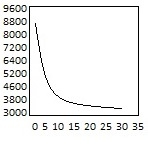
\includegraphics[width=8cm, height=6cm]{ML.jpg}
\end{figure}






\end{document}